\chapter{Resultados}
Neste capítulo serão descritos os resultados obtidos através da simulação da
EDP com a variação de diversos parâmetros. Os parâmetros iniciais escolhidos
para este trabalho foram:
\begin{itemize}
    \item $L_x = 100$m (comprimento do domínio)
    \item $nx = 50$ (número de células)
    \item $\bar{u} = 0.2$m/s (velocidade de escoamento)
    \item $\alpha = 2.0\times10^{-4}$ (coeficiente de difusão)
    \item $c_{\text{ini}} = 1.0$mol/m³ (concentração inicial)
    \item $c_{\text{inj}} = 1.5$mol/m³ (concentração de injeção)
    \item $t_\text{final} = 300$s  (tempo final de simulação)
    \item $\Delta t = 0.1\left( \dfrac{1}{\dfrac{2\alpha}{\Delta x^2} +
           \dfrac{\bar{u}}{\Delta x}} \right) \approx 0.999001$ (passo de tempo)
\end{itemize}

\section{Resultados para variações de $L_x$}
Com a variação de $L_x$, obtiveram-se os seguintes resultados:
\begin{figure}[H]
    \centering
    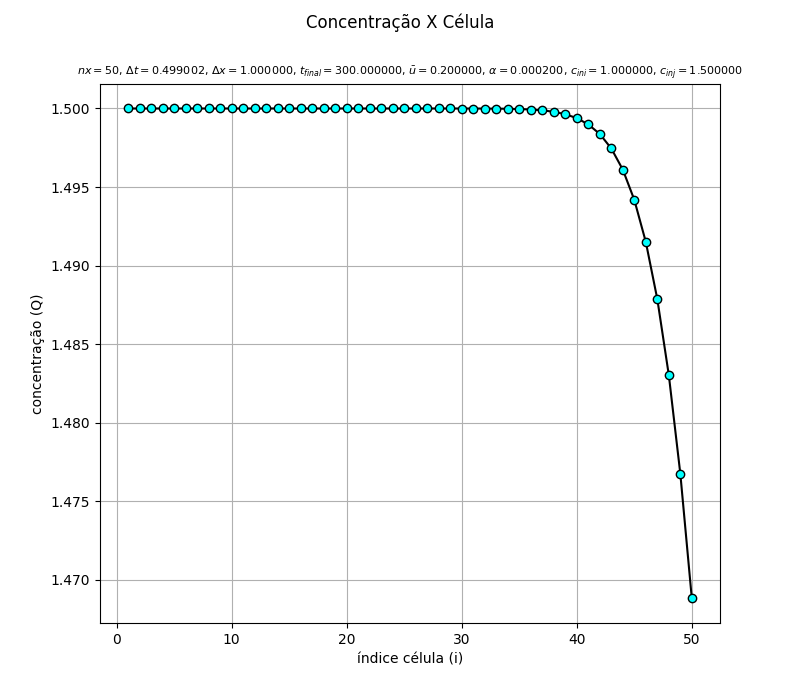
\includegraphics[width=0.7\textwidth]{Lx50}
    \caption{$L_x = 50$m}
\end{figure}
\begin{figure}[H]
    \centering
    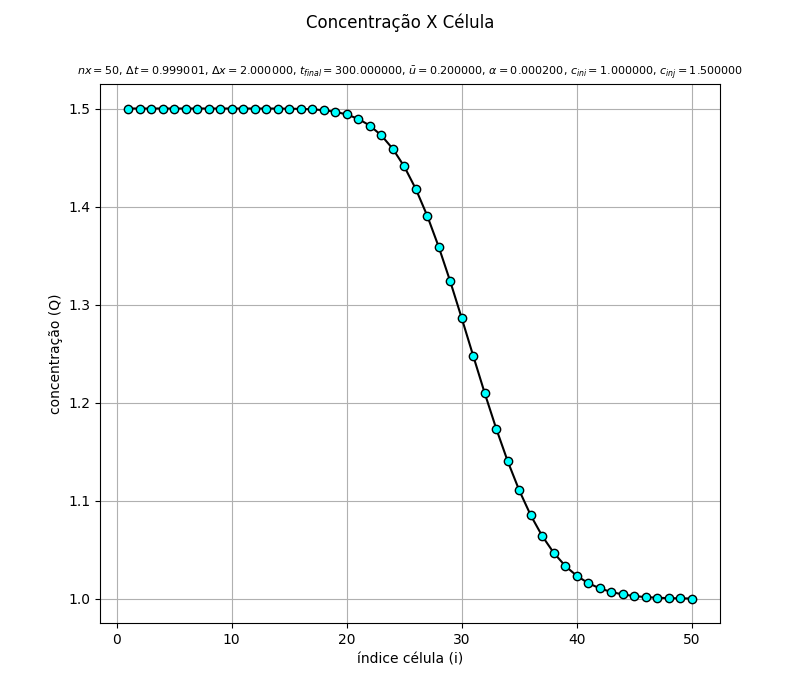
\includegraphics[width=0.7\textwidth]{Lx100}
    \caption{$L_x = 100$m}
\end{figure}
\begin{figure}[H]
    \centering
    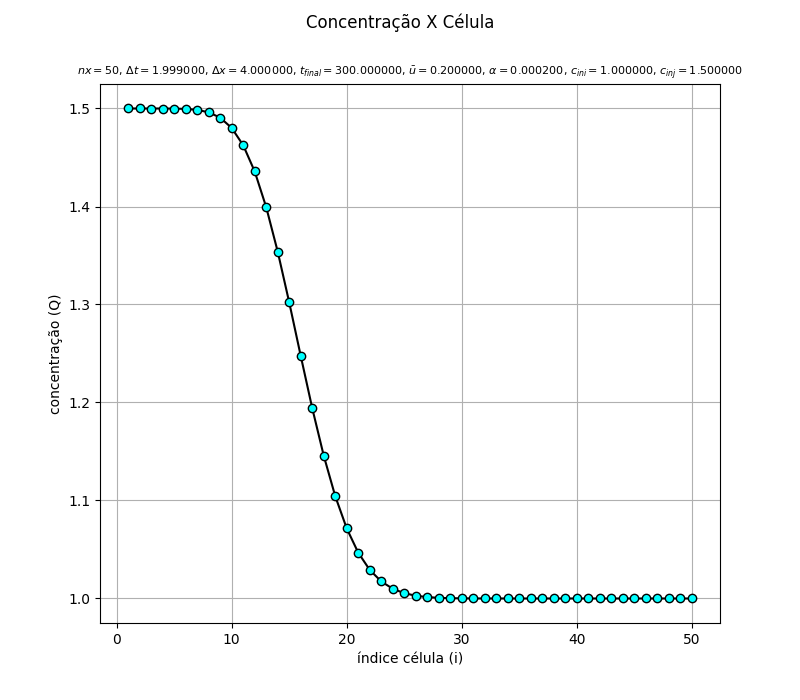
\includegraphics[width=0.7\textwidth]{Lx200}
    \caption{$L_x = 200$m}
\end{figure}
\begin{figure}[H]
    \centering
    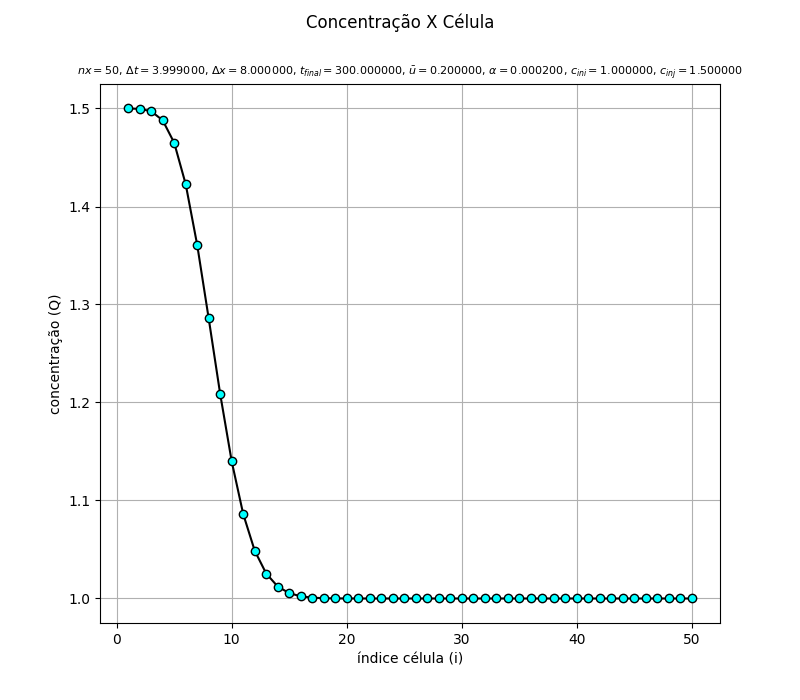
\includegraphics[width=0.7\textwidth]{Lx400}
    \caption{$L_x = 400$m}
\end{figure}

Ao se variar o comprimento do domínio, percebe-se que os efeitos adectivos e
difusivos levam mais tempo para percorrer toda a sua extensão. Sendo assim,
quanto maior o domínio, maior a quantidade de tempo necessária para este
alcançar o equilíbrio.


\section{Resultados para variações de $nx$}
Com a variação de $nx$, obtiveram-se os seguintes resultados:
\begin{figure}[H]
    \centering
    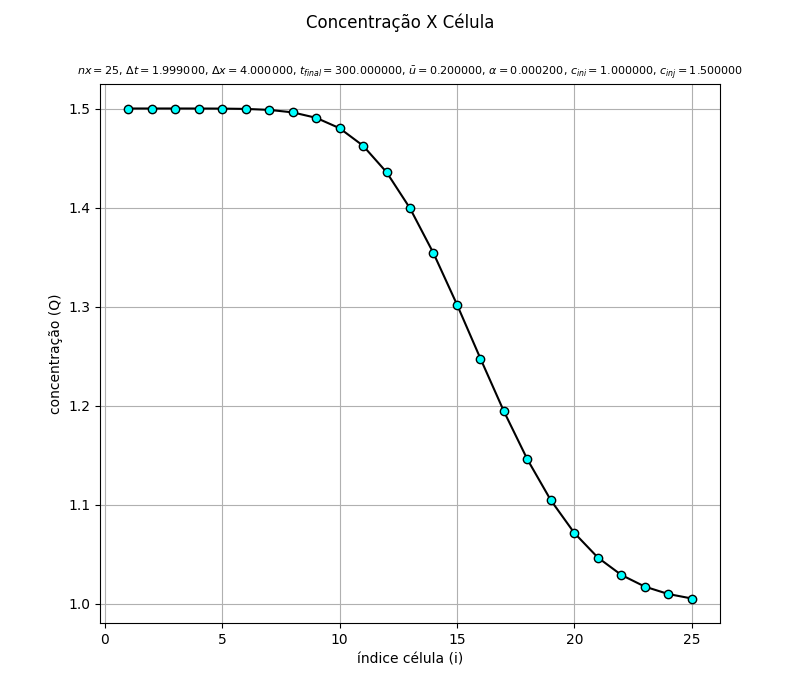
\includegraphics[width=0.7\textwidth]{nx25}
    \caption{$nx = 25$}
\end{figure}
\begin{figure}[H]
    \centering
    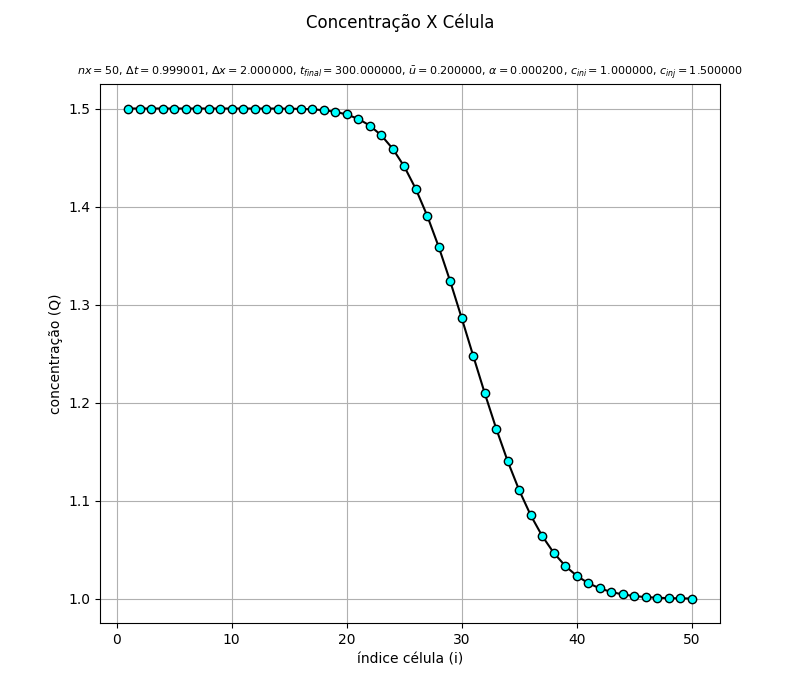
\includegraphics[width=0.7\textwidth]{nx50}
    \caption{$nx = 50$}
\end{figure}
\begin{figure}[H]
    \centering
    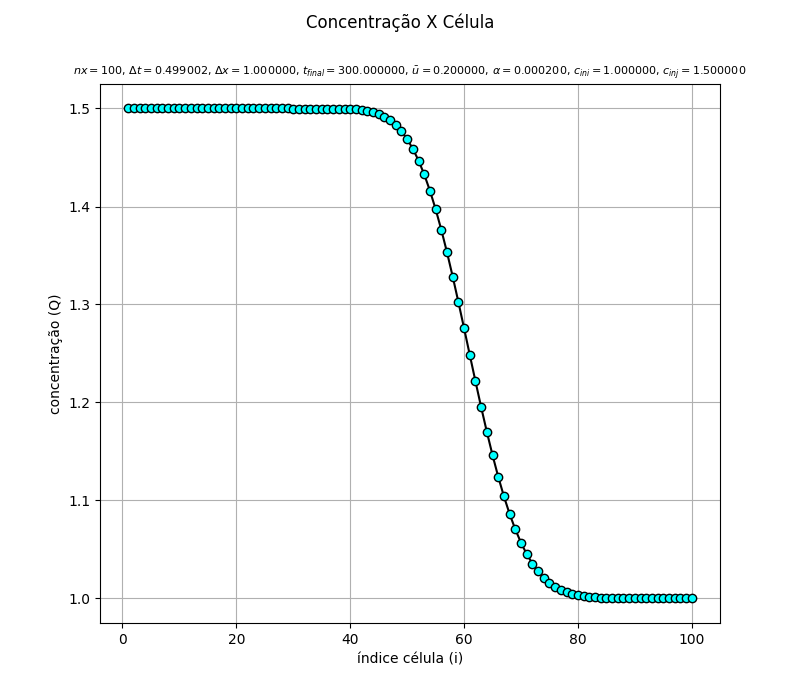
\includegraphics[width=0.7\textwidth]{nx100}
    \caption{$nx = 100$}
\end{figure}

Pode-se observar que a variação do $nx$ resulta em um aumento da resolução do
gráfico. A curva se torna mais detalhada, com mais células descrevendo a
concentração naquela posição do domínio.

\section{Resultados para variações de $\bar{u}$}
Com a variação de $\bar{u}$, obtiveram-se os seguintes resultados:
\begin{figure}[H]
    \centering
    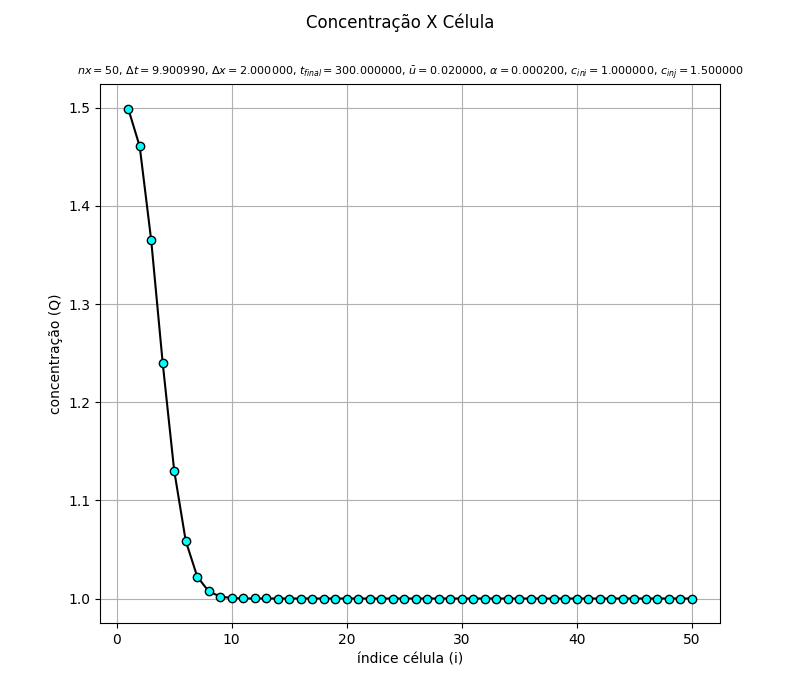
\includegraphics[width=0.7\textwidth]{u2e-2}
    \caption{$\bar{u} = 2\times10^{-2}$m/s}
\end{figure}
\begin{figure}[H]
    \centering
    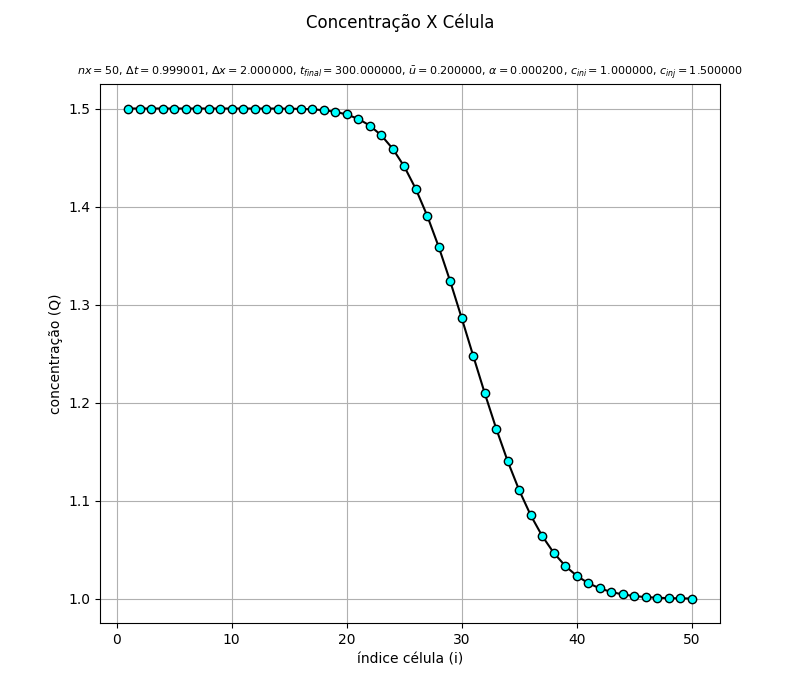
\includegraphics[width=0.7\textwidth]{u2e-1}
    \caption{$\bar{u} = 2\times10^{-1}$m/s}
\end{figure}
\begin{figure}[H]
    \centering
    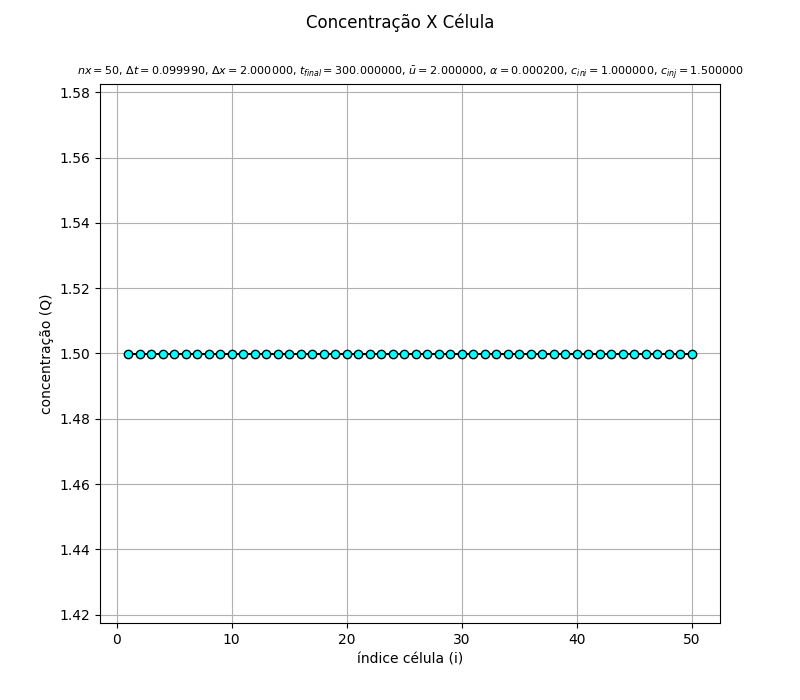
\includegraphics[width=0.7\textwidth]{u2e0}
    \caption{$\bar{u} = 2\times10^{0}$m/s}
\end{figure}

Pode-se observar que o sistema é bastante sensível em relação ao termo
advectivo. Uma mudança na ordem de grandeza da velocidade faz com que este
entre em equilíbrio em uma quantidade de tempo relativamente pequena.

\section{Resultados para variações de $\alpha$}
Com a variação de $\alpha$, obtiveram-se os seguintes resultados:
\begin{figure}[H]
    \centering
    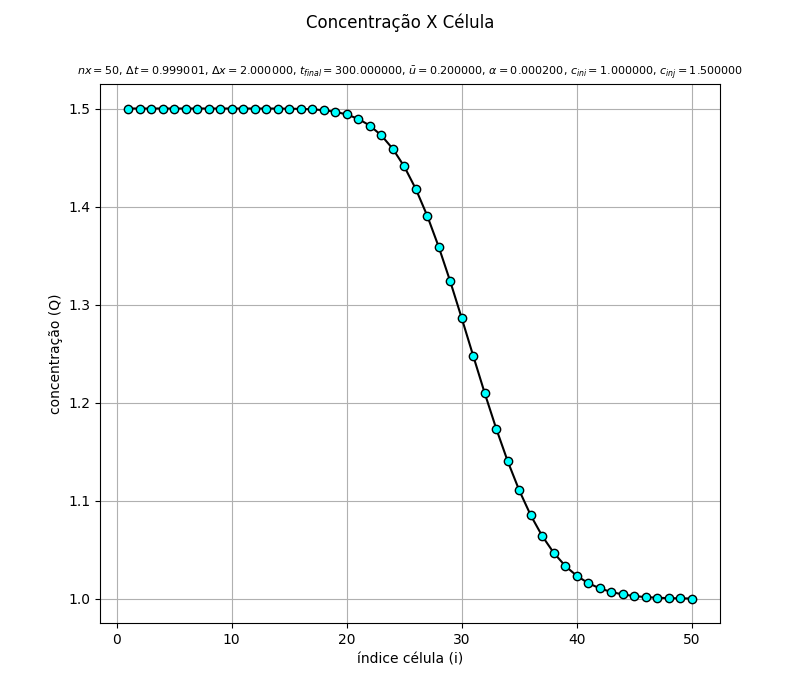
\includegraphics[width=0.7\textwidth]{alpha2e-4}
    \caption{$\alpha = 2.0\times10^{-4}$}
\end{figure}
\begin{figure}[H]
    \centering
    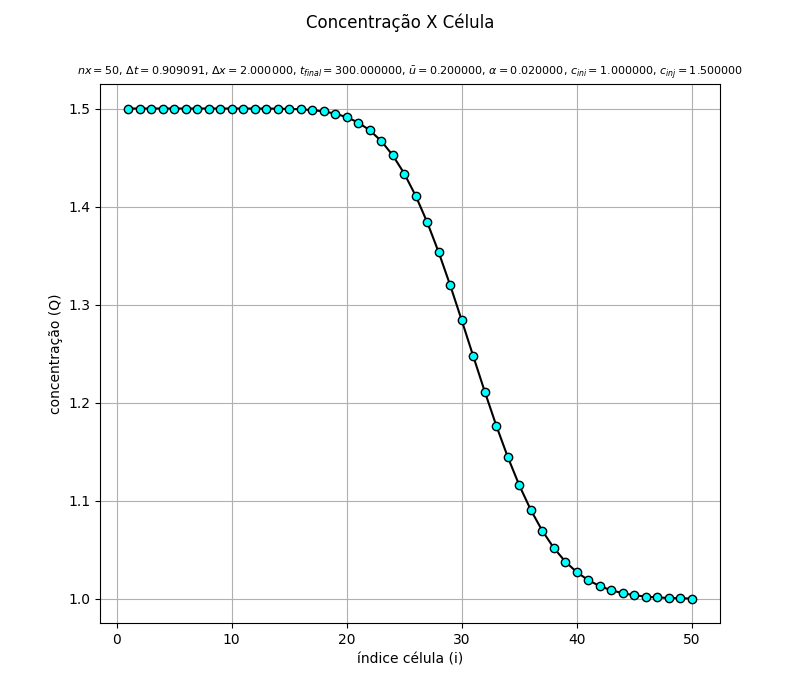
\includegraphics[width=0.7\textwidth]{alpha2e-2}
    \caption{$\alpha = 2.0\times10^{-2}$}
\end{figure}
\begin{figure}[H]
    \centering
    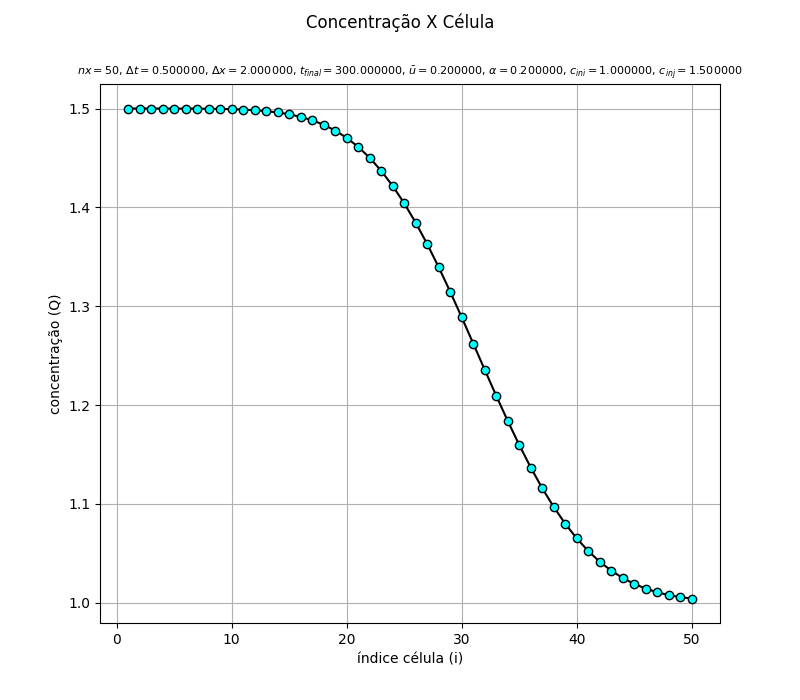
\includegraphics[width=0.7\textwidth]{alpha2e-1}
    \caption{$\alpha = 2.0\times10^{-1}$}
\end{figure}
\begin{figure}[H]
    \centering
    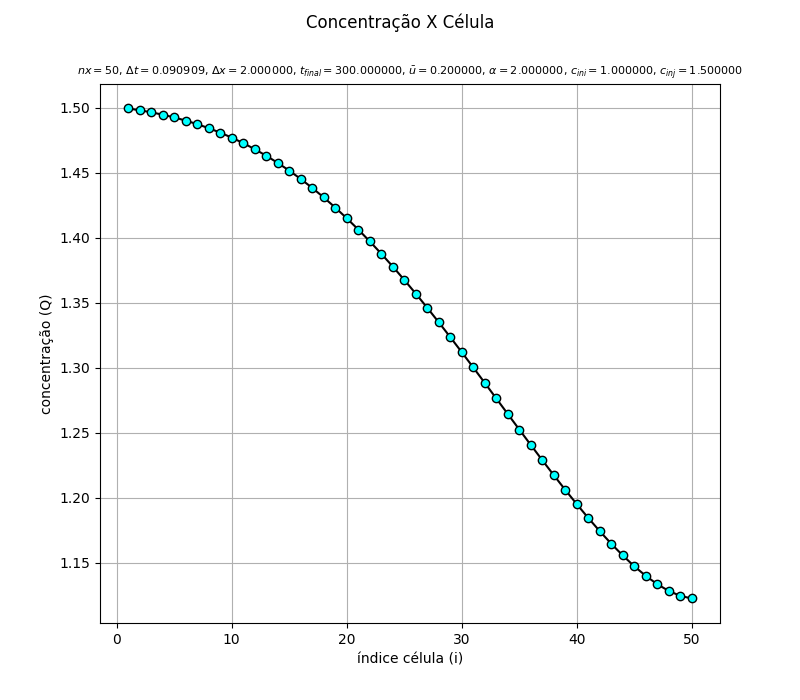
\includegraphics[width=0.7\textwidth]{alpha2e0}
    \caption{$\alpha = 2.0\times10^{0}$}
\end{figure}

Nota-se que a presença do efeito difusivo é quase desprezível a concentrações
na ordem de $10^{-4}$. Para $\alpha \geq 1$, porém, o efeito difusivo passa a
ter uma presença significativa sobre o sistema, devendo assim ser levado em
conta na modelagem de um problema real de engenharia.

\section{Resultados para $\bar{u}=0$ e variações de $\alpha$}
No caso especial onde há uma ausência do termo advectivo, obtiveram-se os
seguintes resultados:
\begin{figure}[H]
    \centering
    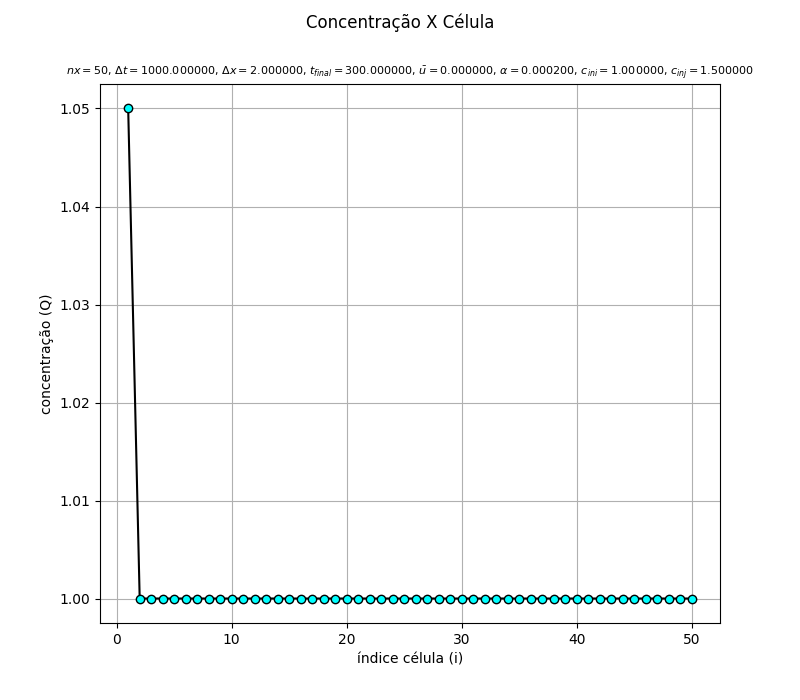
\includegraphics[width=0.7\textwidth]{u0&alpha2e-4}
    \caption{$\bar{u} = 0\ \&\ \alpha = 2.0\times10^{-4}$}
\end{figure}
\begin{figure}[H]
    \centering
    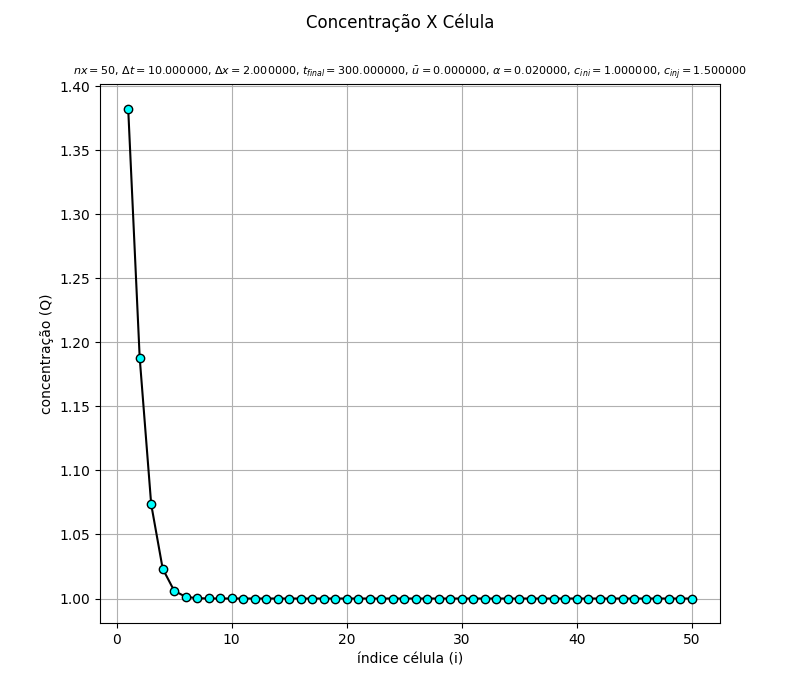
\includegraphics[width=0.7\textwidth]{u0&alpha2e-2}
    \caption{$\bar{u} = 0\ \&\ \alpha = 2.0\times10^{-2}$}
\end{figure}
\begin{figure}[H]
    \centering
    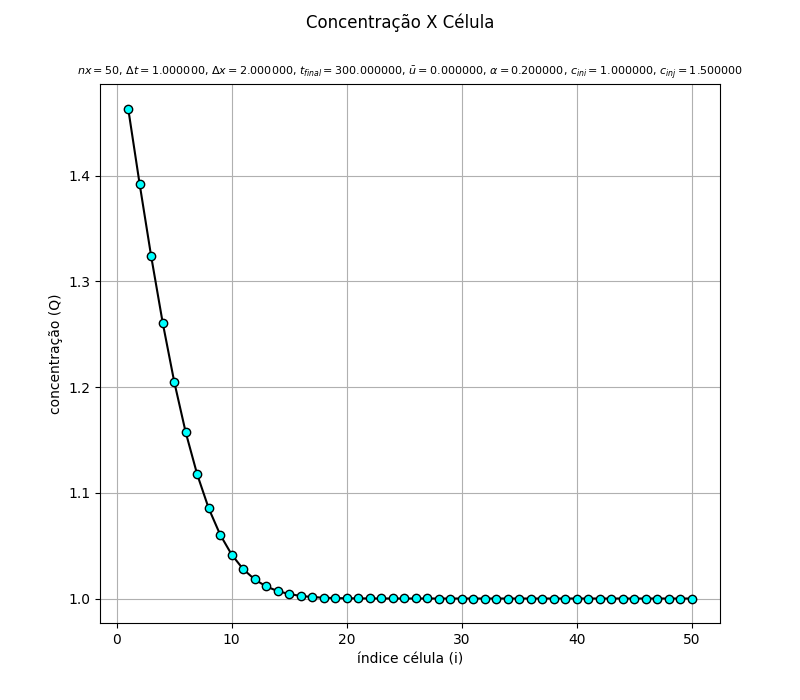
\includegraphics[width=0.7\textwidth]{u0&alpha2e-1}
    \caption{$\bar{u} = 0\ \&\ \alpha = 2.0\times10^{-1}$}
\end{figure}
\begin{figure}[H]
    \centering
    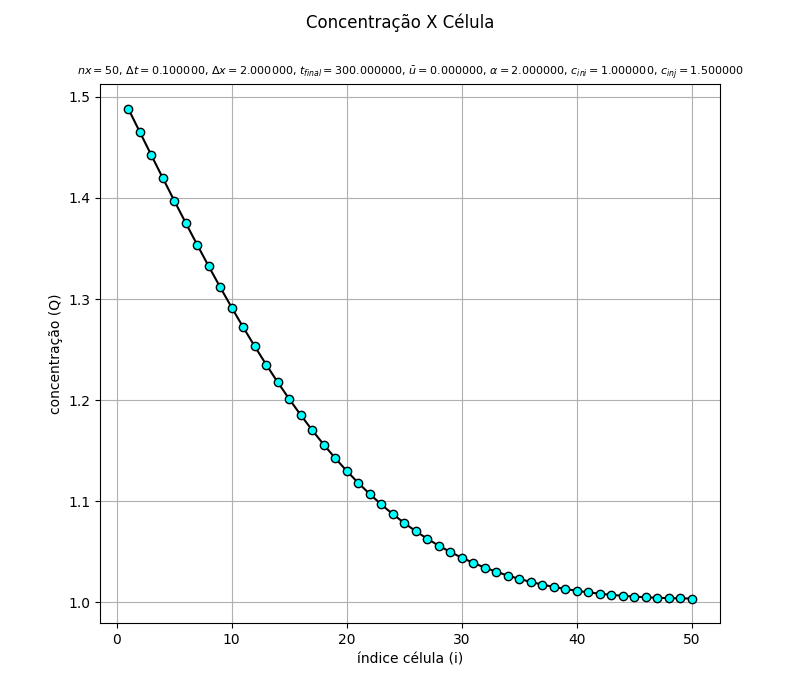
\includegraphics[width=0.7\textwidth]{u0&alpha2e0}
    \caption{$\bar{u} = 0\ \&\ \alpha = 2.0\times10^{0}$}
\end{figure}

Com a ausência de um termo advectivo, o sistema leva bastante tempo para
alcançar a estabilidade dado valores de $\alpha \leq 10^{-2}$, pois a
influência de um dado volume sobre os seus vizinhos é bastante pequeno. Com
valores maiores, porém, os efeitos difusivos podem ser claramente apreciados, e
a diferença de concentrações se propaga pelo sistema rapidamente.

\section{Resultados para variações de $c_\text{ini}$}
Com a variação de $c_{ini}$, obtiveram-se os seguintes resultados:
\begin{figure}[H]
    \centering
    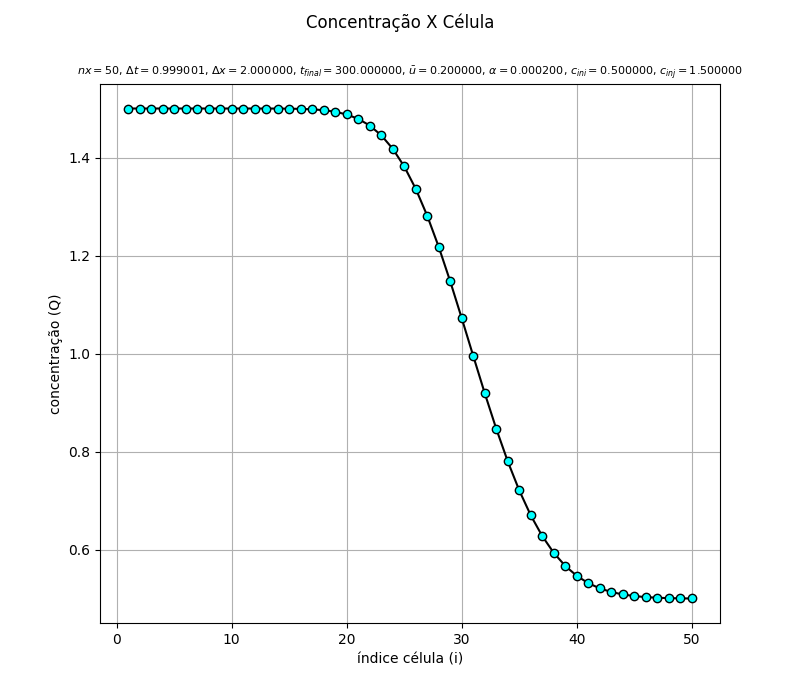
\includegraphics[width=0.7\textwidth]{c_ini0.5}
    \caption{$c_\text{ini} = 0.5$mol/m³}
\end{figure}
\begin{figure}[H]
    \centering
    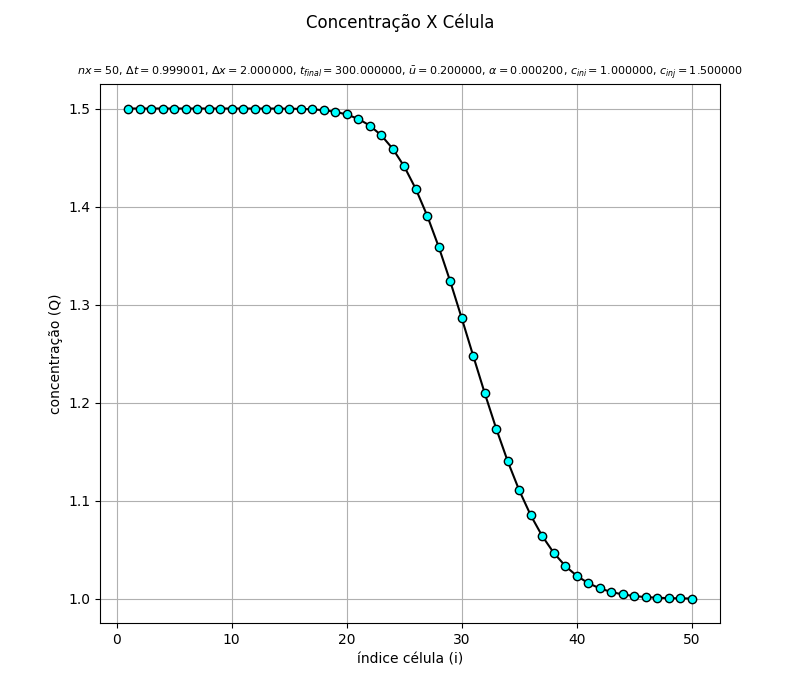
\includegraphics[width=0.7\textwidth]{c_ini1}
    \caption{$c_\text{ini} = 1.0$mol/m³}
\end{figure}
\begin{figure}[H]
    \centering
    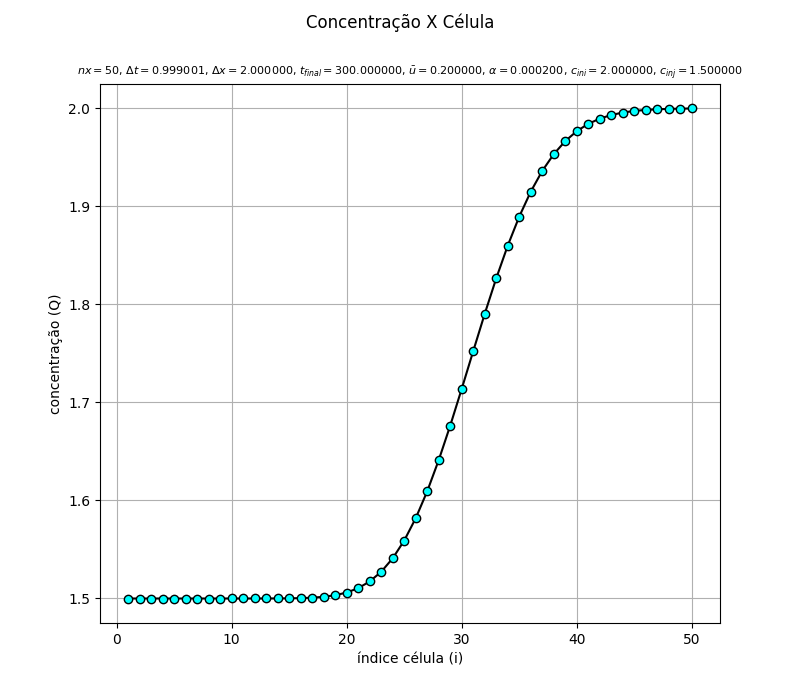
\includegraphics[width=0.7\textwidth]{c_ini2}
    \caption{$c_\text{ini} = 2.0$mol/m³}
\end{figure}

Para uma variação da concentração inicial, nota-se que os volumes mais
próximos do contorno direito mantém esse valor para um tempo de simulação no
qual os efeitos advectivos e difusivos não foram suficientes para
influenciá-los. Sendo assim, para uma concentração inicial $c_{ini}$ maior que
a concentração de injeção $c_{inj}$ o gráfico acaba se invertendo.

\section{Resultados para variações de $c_\text{inj}$}
Com a variação de $c_\text{inj}$, obtiveram-se os seguintes resultados:
\begin{figure}[H]
    \centering
    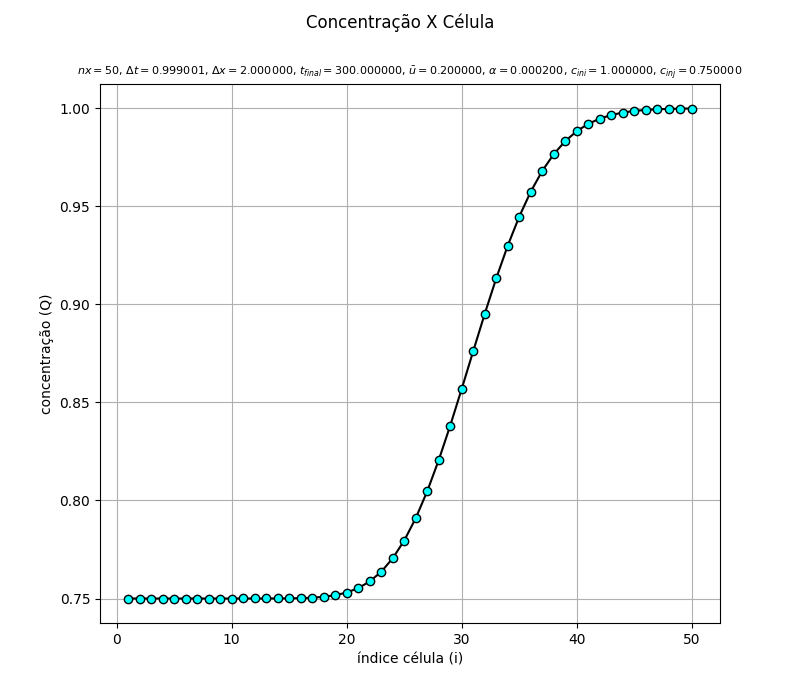
\includegraphics[width=0.7\textwidth]{c_inj0.75}
    \caption{$c_\text{inj} = 0.75$mol/m³}
\end{figure}
\begin{figure}[H]
    \centering
    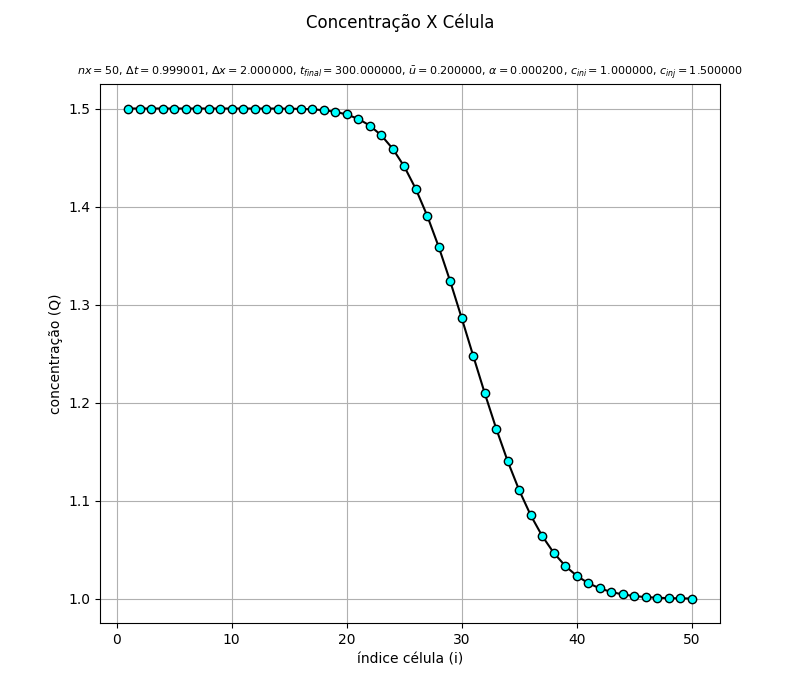
\includegraphics[width=0.7\textwidth]{c_inj1.5}
    \caption{$c_\text{inj} = 1.5$mol/m³}
\end{figure}
\begin{figure}[H]
    \centering
    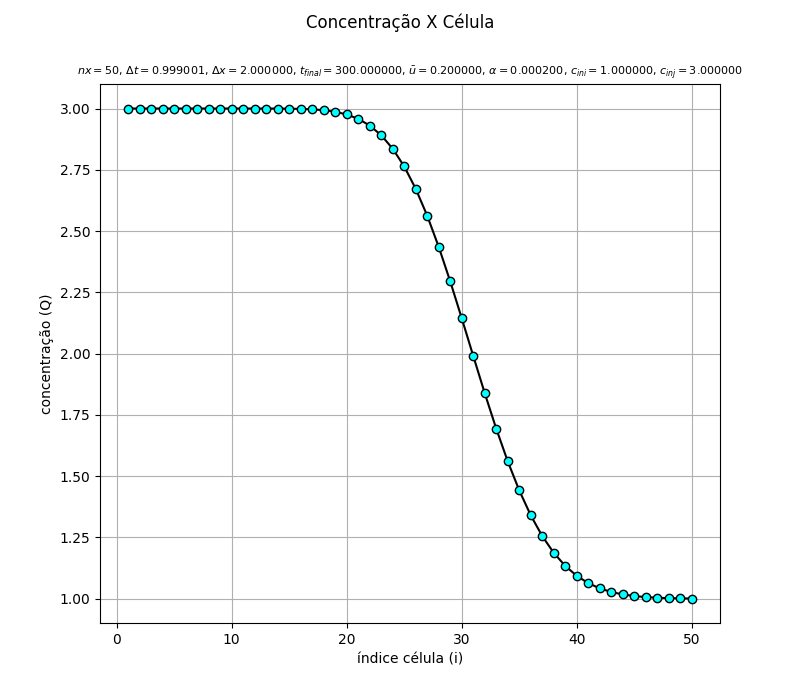
\includegraphics[width=0.7\textwidth]{c_inj3}
    \caption{$c_\text{inj} = 3.0$mol/m³}
\end{figure}

Para uma variação da concentração de injeção, tem-se a situação oposta da seção
anterior: volumes próximos ao contorno esquerdo sofrem influência quase que
imediata da concentração de injeção, enquanto volumes distantes levam mais
tempo para serem influenciados por seus vizinhos.

\section{Resultados para variações de $t_\text{final}$}
Com a variação de $t_\text{final}$, obtiveram-se os seguintes resultados:
\begin{figure}[H]
    \centering
    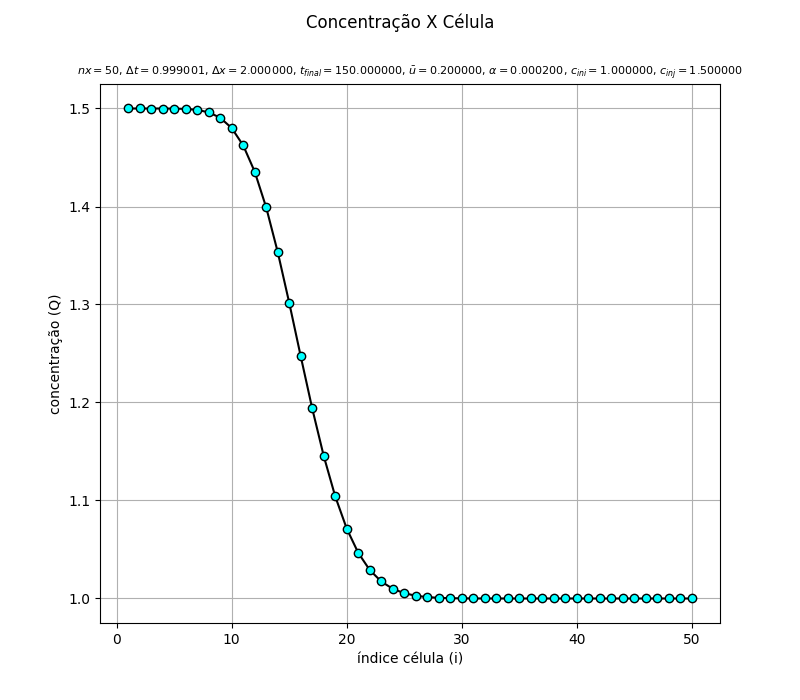
\includegraphics[width=0.7\textwidth]{t_final150}
    \caption{$t_\text{final} = 150$s}
\end{figure}
\begin{figure}[H]
    \centering
    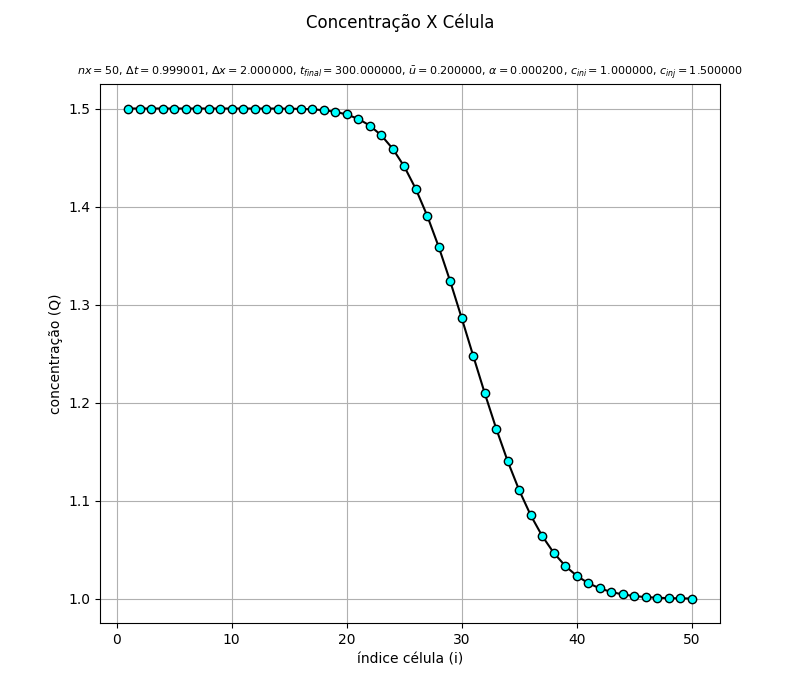
\includegraphics[width=0.7\textwidth]{t_final300}
    \caption{$t_\text{final} = 300$s}
\end{figure}
\begin{figure}[H]
    \centering
    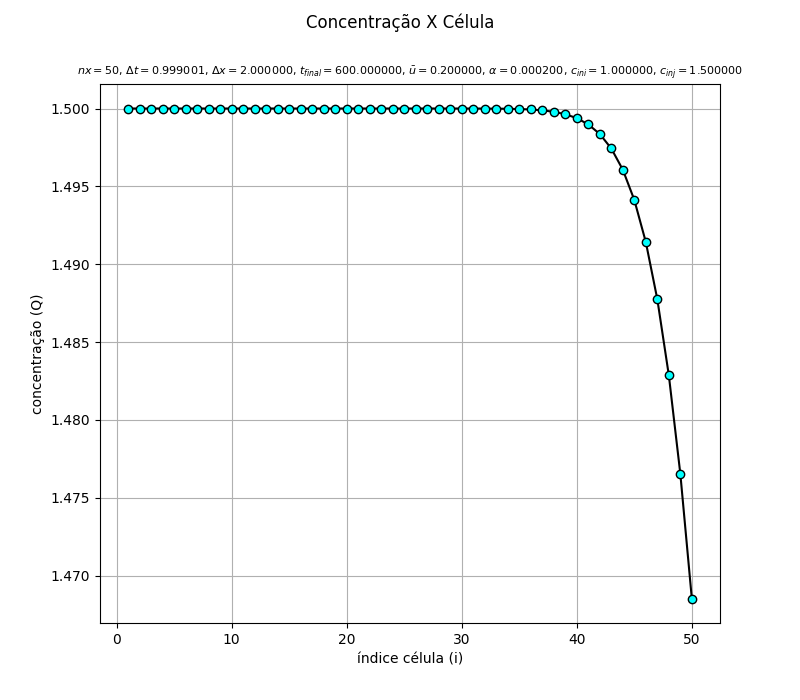
\includegraphics[width=0.7\textwidth]{t_final600}
    \caption{$t_\text{final} = 600$s}
\end{figure}
\begin{figure}[H]
    \centering
    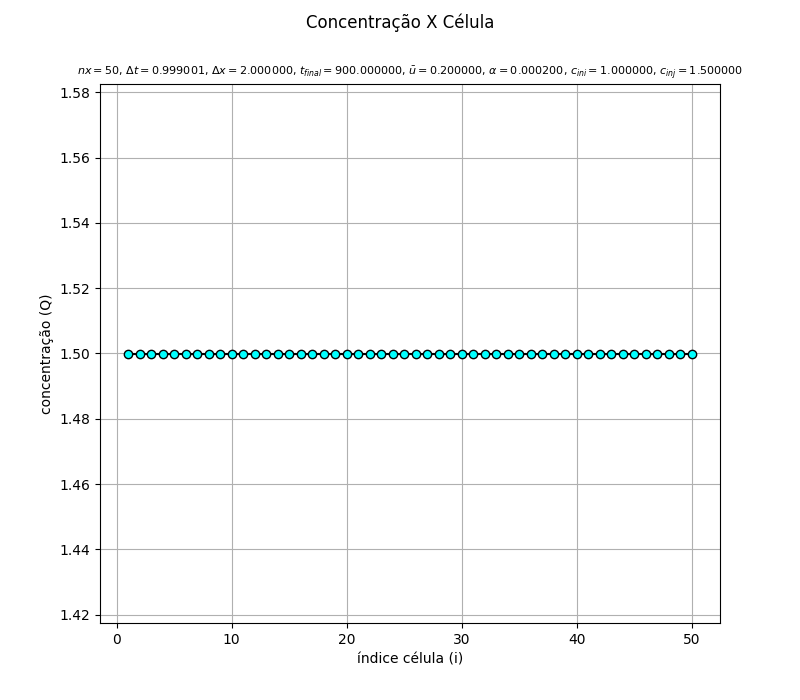
\includegraphics[width=0.7\textwidth]{t_final900}
    \caption{$t_\text{final} = 900$s}
\end{figure}

Ao variar o tempo de simulação, nota-se que o sistema tende ao equilíbrio dado
um tempo longo o suficiente para os efeitos difusivos e advectivos
influenciarem todos os volumes de seu domínio.



